\documentclass{memoir}


\usepackage{hyperref}

%%% Page geometry
\usepackage[
  paperwidth=8.5in,
  paperheight=8.5in,
  layoutwidth=8.5in,
  layoutheight=8.5in,
  vmargin=0.5in,
  outer=0.5in,
  inner=0.75in,
  includeheadfoot,
  twoside
]{geometry}

%%% Font
\usepackage{fontspec}
\setmainfont{Gentium Book Basic}
\newfontfamily\titlefamily{Ubuntu}
\newfontface\titlefont{Ubuntu}
\newfontface\urlfont{Ubuntu Mono}

%%% Graphics
\usepackage{graphicx}

%%% Table of contents
\renewcommand{\contentsname}{\titlefamily FOOD}
% flushright chapter numbers
\renewcommand{\cftchapterfont}{\normalfont\titlefamily\bfseries}
\renewcommand{\cftsectionfont}{\normalfont\titlefamily}
\setlength{\cftbeforechapterskip}{1.8ex}
\setlength{\cftbeforesectionskip}{0.75ex}
\renewcommand{\cftdot}{\small{$\cdot$}}
\renewcommand{\cftchapterdotsep}{10000}
\renewcommand{\cftsectiondotsep}{3}
\renewcommand*\tocheadstart{}{}

%%% Headers and chapters
\let\footruleskip\undefined
\DisemulatePackage{setspace}
\usepackage[pagestyles]{titlesec}
\usepackage{fancyhdr}
\setlength{\headheight}{15.2pt}
% arcana style with fancy headers and chapter headings
\fancypagestyle{fancyplain}{
  % headers
  \fancyhf{}
  \fancyhf[FRO,FLE]{\titlefamily\thepage}
  \fancyhf[HLE]{\titlefamily\chaptertitle}
  \fancyhf[HRO]{\titlefamily MEALTIME WITH MADDY}

  %%% With inner headers
  % \fancyhf[HLE,HRO]{\titlefamily\textit{Arcana}}
  % \fancyhf[HLO]{\pfdfamily\itshape\arcstoryauthor}
  % \fancyhf[HRE]{\titlefamily\ifthenelse{\equal{\arcsubheading}{}}{\chaptertitle}{\chaptertitle\normalfont\ --- {\pfdfamily\arcsubheading}}}
  \renewcommand{\headrulewidth}{0.5pt}
  \renewcommand{\chapterheadstart}{}
  \renewcommand{\printchaptername}{}
  \renewcommand{\chapternamenum}{}
  \renewcommand{\printchapternum}{}
  \renewcommand{\afterchapternum}{}
  \renewcommand{\printchaptertitle}[1]{%
  \titlefamily\raggedright\Huge{##1}}
  \renewcommand{\afterchaptertitle}{%
  \vskip\onelineskip \hrule\vskip\onelineskip}
  \setbeforesecskip{1ex}
  \setaftersecskip{1ex}
  \setlength{\parskip}{0pt}
}
\fancypagestyle{afterword}{
  % headers - same for arcana pagestyle
  \fancyhf{}
  \fancyhf[FRO,FLE]{\titlefamily\thepage}
  \fancyhf[HLE,HRO]{\titlefamily MEALTIME WITH MADDY}
  % chapter headings with card names - same for arcana pagestyle
  \renewcommand{\headrulewidth}{0.5pt}
  \renewcommand{\chapterheadstart}{}
  \renewcommand{\printchaptername}{}
  \renewcommand{\chapternamenum}{}
  \renewcommand{\printchapternum}{}
  \renewcommand{\afterchapternum}{}
  % this is the only changed command from arcana: remove \thechapter from chapter header
  \renewcommand{\printchaptertitle}[1]{%
  \titlefamily\raggedright\Huge{\hspace{2em} ##1}}
  \renewcommand{\afterchaptertitle}{%
  \vskip\onelineskip \hrule\vskip\onelineskip}
  \setbeforesecskip{1ex}
  \setaftersecskip{1ex}
}
% plain style with only page num
\fancypagestyle{plain}{
  \fancyhf{}
  \renewcommand{\headrulewidth}{0pt}
  \renewcommand{\footrulewidth}{0pt}
  \fancyhf[FRO,FLE]{\thepage}
}
% single space after periods
\frenchspacing
% Attempt justification at all costs
\sloppy


\begin{document}
\frontmatter

\pagestyle{empty}
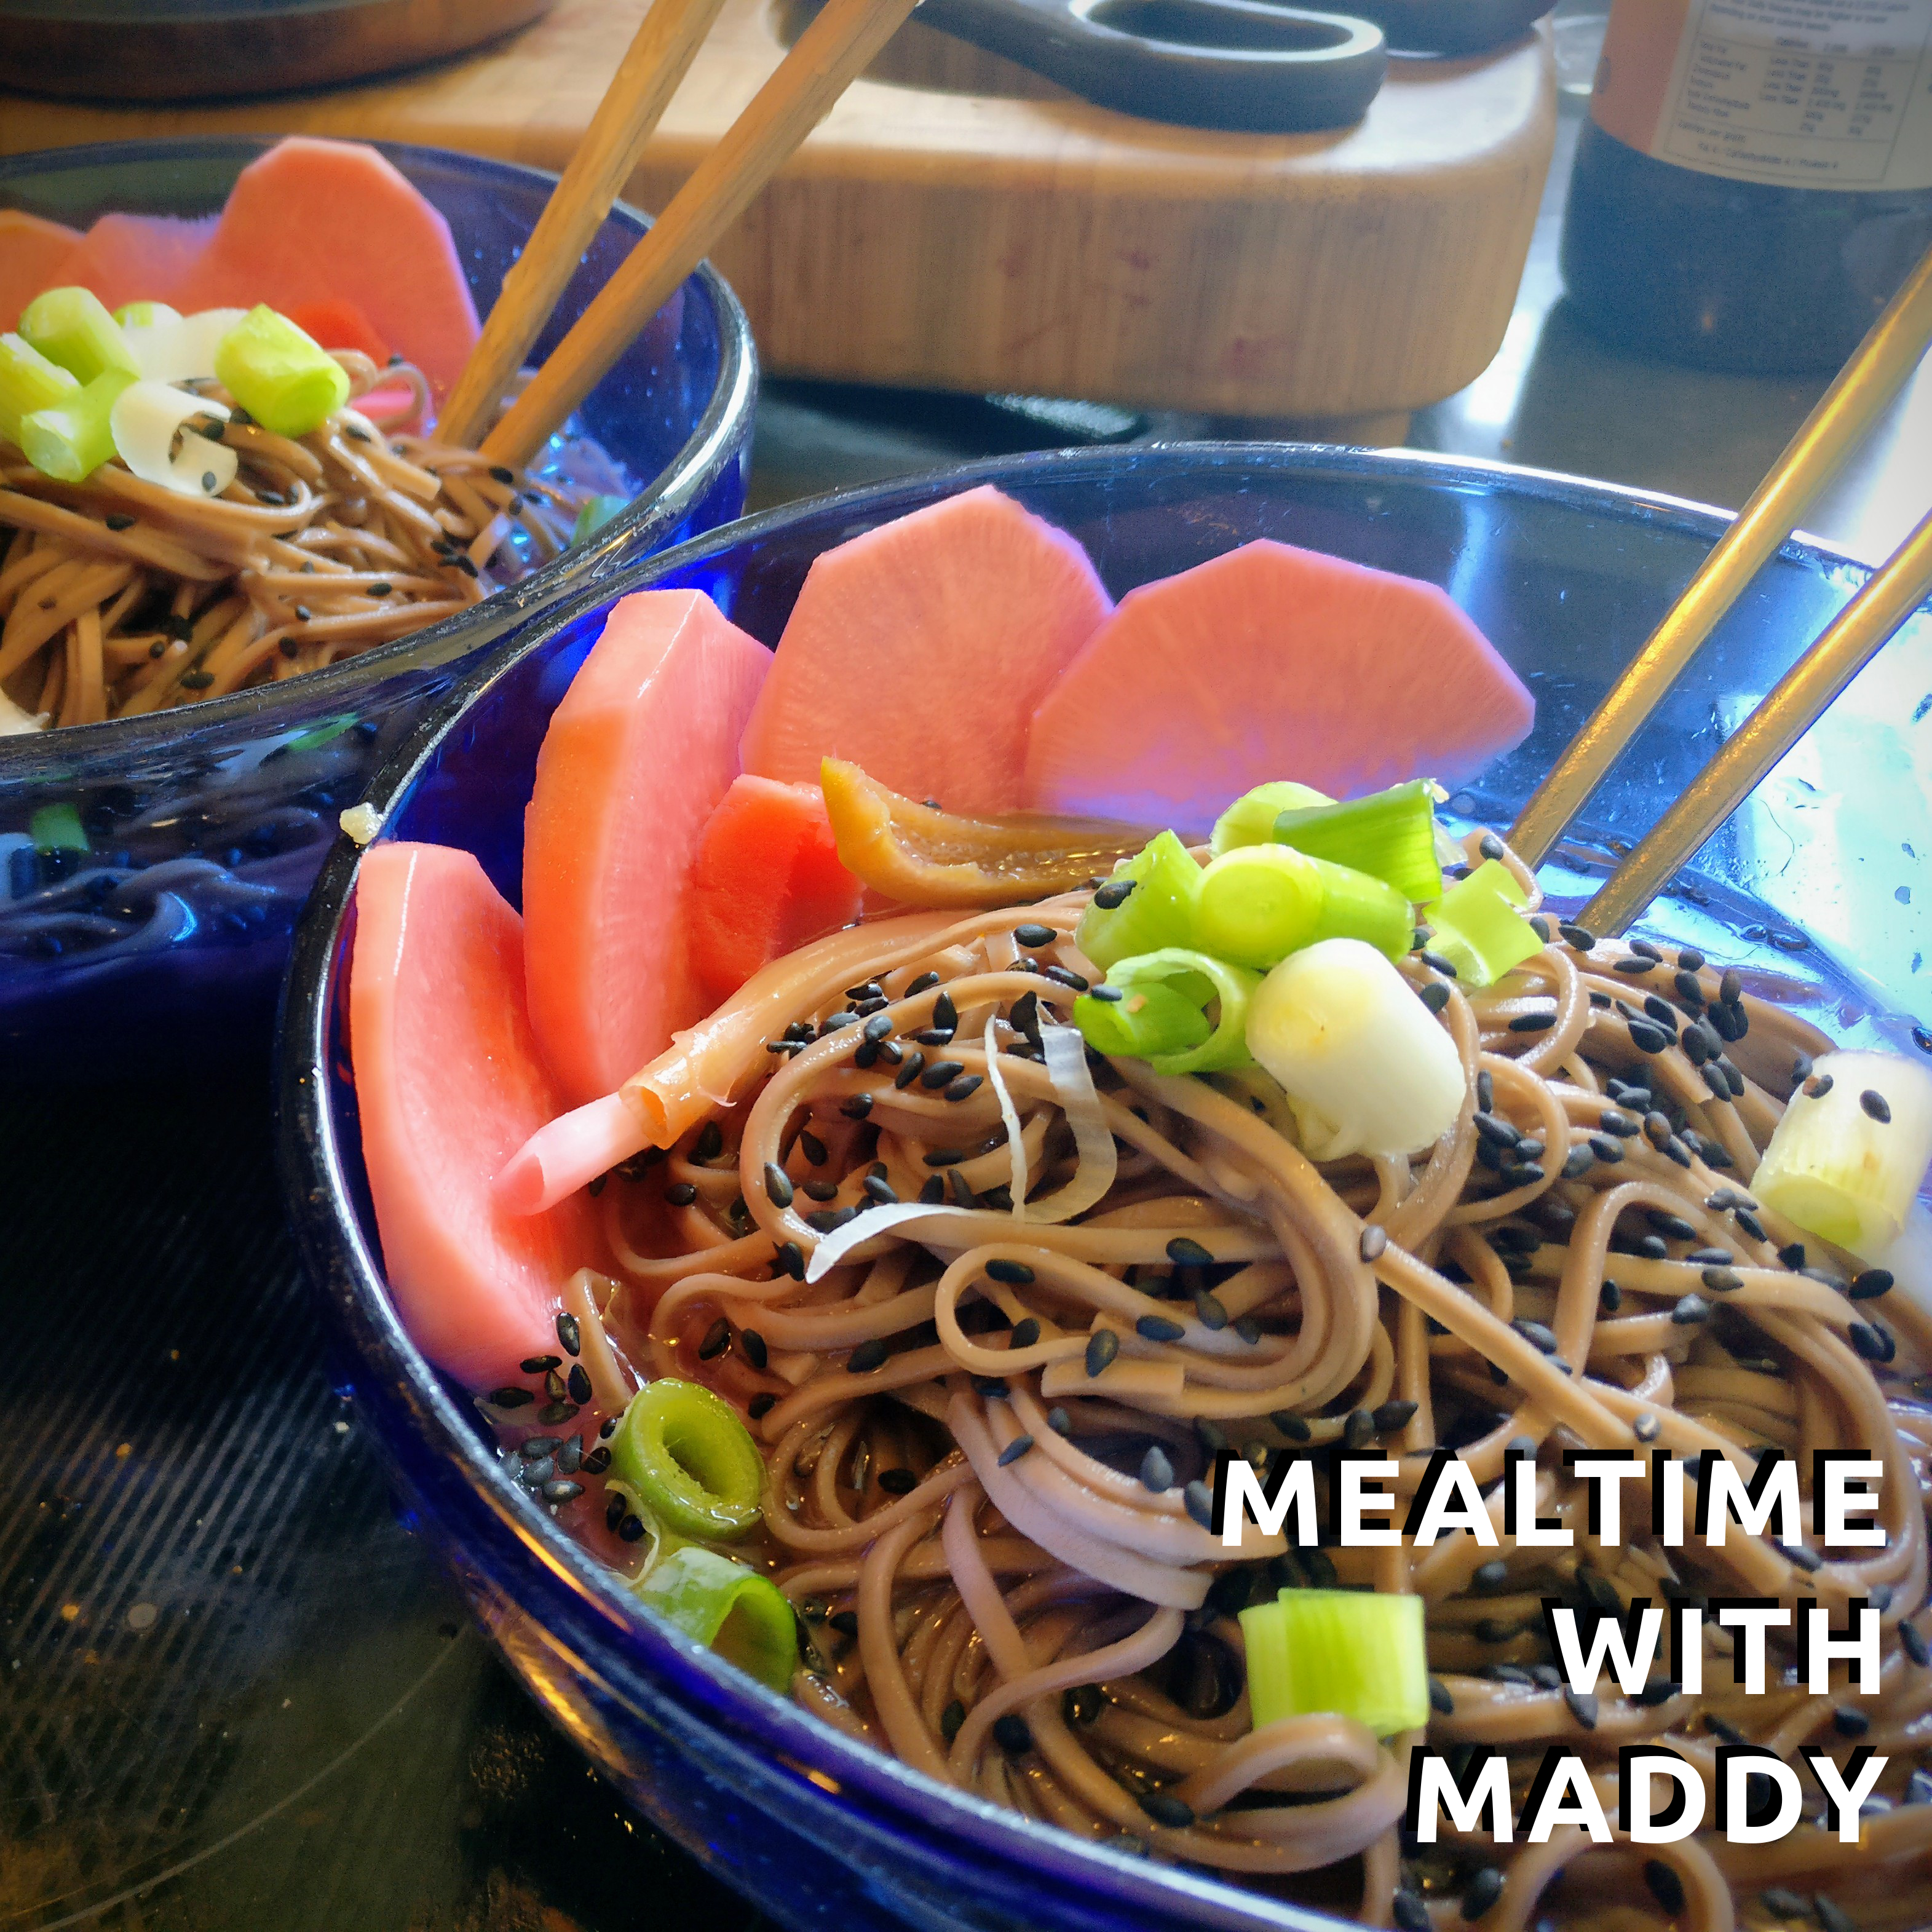
\includegraphics[width=6.5in]{inner-cover.png}
\newpage

\null
\vfill

\titlefont MEALTIME WITH MADDY \copyright\ Madison Scott-Clary, 2017

\vspace{1ex}

This work is licensed under a Creative Commons Attribution-ShareAlike 4.0 International License

\vspace{1ex}

For more information, see \mbox{\urlfont https://creativecommons.org/licenses/by-sa/4.0/}

\vspace{1cm}

This book is part of an evolving project. To keep up to date and see future recipes and hollering, visit \mbox{\urlfont http://mealtime.with.maddypa.ws}

\vfill
\newpage

\pagestyle{fancyplain}
\tableofcontents*

\normalfont

\chapter*{Dedication}

\begin{verse}
  To the polycule\\
  \vin JD and Robin and Lexy\\
  To Jenn\\
  To the dogs\\
  \vin Zephyr and Falcon\\
  And to the idea\\
  \vin If not exactly the implementation\\
  \vin \vin Of Twitter.
\end{verse}

\chapter[About]{About}

\mainmatter

\chapter*{Bananas Foster}
\renewcommand{\chaptertitle}{Bananas Foster}
\addcontentsline{toc}{chapter}{\hspace{1.5ex}Bananas Foster}

\includegraphics[height=\textwidth-1.3in]{food/bananas-foster/images/hi-res/01.jpg}
\newpage
\includegraphics[width=\textwidth]{food/bananas-foster/images/hi-res/02.jpg}
\newpage
\includegraphics[width=\textwidth]{food/bananas-foster/images/hi-res/03.jpg}
\newpage
\includegraphics[width=\textwidth]{food/bananas-foster/images/hi-res/04.jpg}
\newpage
\includegraphics[width=\textwidth]{food/bananas-foster/images/hi-res/05.jpg}
\newpage
\includegraphics[width=\textwidth]{food/bananas-foster/images/hi-res/06.jpg}
\newpage
\includegraphics[height=\textheight]{food/bananas-foster/images/hi-res/07.jpg}
\newpage
\includegraphics[width=\textwidth]{food/bananas-foster/images/hi-res/08.jpg}
\newpage
\includegraphics[width=\textwidth]{food/bananas-foster/images/hi-res/09.jpg}
\newpage
\includegraphics[width=\textwidth]{food/bananas-foster/images/hi-res/10.jpg}


\chapter*{Dal}
\renewcommand{\chaptertitle}{Dal}
\addcontentsline{toc}{chapter}{\hspace{1.5ex}Dal}


\chapter*{Bananas Foster}
\renewcommand{\chaptertitle}{Bananas Foster}
\addcontentsline{toc}{chapter}{\hspace{1.5ex}Bananas Foster}

\includegraphics[height=\textwidth-1.3in]{food/bananas-foster/images/hi-res/01.jpg}
\newpage
\includegraphics[width=\textwidth]{food/bananas-foster/images/hi-res/02.jpg}
\newpage
\includegraphics[width=\textwidth]{food/bananas-foster/images/hi-res/03.jpg}
\newpage
\includegraphics[width=\textwidth]{food/bananas-foster/images/hi-res/04.jpg}
\newpage
\includegraphics[width=\textwidth]{food/bananas-foster/images/hi-res/05.jpg}
\newpage
\includegraphics[width=\textwidth]{food/bananas-foster/images/hi-res/06.jpg}
\newpage
\includegraphics[height=\textheight]{food/bananas-foster/images/hi-res/07.jpg}
\newpage
\includegraphics[width=\textwidth]{food/bananas-foster/images/hi-res/08.jpg}
\newpage
\includegraphics[width=\textwidth]{food/bananas-foster/images/hi-res/09.jpg}
\newpage
\includegraphics[width=\textwidth]{food/bananas-foster/images/hi-res/10.jpg}


\chapter*{Bananas Foster}
\renewcommand{\chaptertitle}{Bananas Foster}
\addcontentsline{toc}{chapter}{\hspace{1.5ex}Bananas Foster}

\includegraphics[height=\textwidth-1.3in]{food/bananas-foster/images/hi-res/01.jpg}
\newpage
\includegraphics[width=\textwidth]{food/bananas-foster/images/hi-res/02.jpg}
\newpage
\includegraphics[width=\textwidth]{food/bananas-foster/images/hi-res/03.jpg}
\newpage
\includegraphics[width=\textwidth]{food/bananas-foster/images/hi-res/04.jpg}
\newpage
\includegraphics[width=\textwidth]{food/bananas-foster/images/hi-res/05.jpg}
\newpage
\includegraphics[width=\textwidth]{food/bananas-foster/images/hi-res/06.jpg}
\newpage
\includegraphics[height=\textheight]{food/bananas-foster/images/hi-res/07.jpg}
\newpage
\includegraphics[width=\textwidth]{food/bananas-foster/images/hi-res/08.jpg}
\newpage
\includegraphics[width=\textwidth]{food/bananas-foster/images/hi-res/09.jpg}
\newpage
\includegraphics[width=\textwidth]{food/bananas-foster/images/hi-res/10.jpg}


\chapter*{Tabbouleh}
\renewcommand{\chaptertitle}{Tabbouleh}
\addcontentsline{toc}{chapter}{\hspace{1.5ex}Tabbouleh}

TIP fried


\chapter*{Bananas Foster}
\renewcommand{\chaptertitle}{Bananas Foster}
\addcontentsline{toc}{chapter}{\hspace{1.5ex}Bananas Foster}

\includegraphics[height=\textwidth-1.3in]{food/bananas-foster/images/hi-res/01.jpg}
\newpage
\includegraphics[width=\textwidth]{food/bananas-foster/images/hi-res/02.jpg}
\newpage
\includegraphics[width=\textwidth]{food/bananas-foster/images/hi-res/03.jpg}
\newpage
\includegraphics[width=\textwidth]{food/bananas-foster/images/hi-res/04.jpg}
\newpage
\includegraphics[width=\textwidth]{food/bananas-foster/images/hi-res/05.jpg}
\newpage
\includegraphics[width=\textwidth]{food/bananas-foster/images/hi-res/06.jpg}
\newpage
\includegraphics[height=\textheight]{food/bananas-foster/images/hi-res/07.jpg}
\newpage
\includegraphics[width=\textwidth]{food/bananas-foster/images/hi-res/08.jpg}
\newpage
\includegraphics[width=\textwidth]{food/bananas-foster/images/hi-res/09.jpg}
\newpage
\includegraphics[width=\textwidth]{food/bananas-foster/images/hi-res/10.jpg}


\chapter*{Bananas Foster}
\renewcommand{\chaptertitle}{Bananas Foster}
\addcontentsline{toc}{chapter}{\hspace{1.5ex}Bananas Foster}

\includegraphics[height=\textwidth-1.3in]{food/bananas-foster/images/hi-res/01.jpg}
\newpage
\includegraphics[width=\textwidth]{food/bananas-foster/images/hi-res/02.jpg}
\newpage
\includegraphics[width=\textwidth]{food/bananas-foster/images/hi-res/03.jpg}
\newpage
\includegraphics[width=\textwidth]{food/bananas-foster/images/hi-res/04.jpg}
\newpage
\includegraphics[width=\textwidth]{food/bananas-foster/images/hi-res/05.jpg}
\newpage
\includegraphics[width=\textwidth]{food/bananas-foster/images/hi-res/06.jpg}
\newpage
\includegraphics[height=\textheight]{food/bananas-foster/images/hi-res/07.jpg}
\newpage
\includegraphics[width=\textwidth]{food/bananas-foster/images/hi-res/08.jpg}
\newpage
\includegraphics[width=\textwidth]{food/bananas-foster/images/hi-res/09.jpg}
\newpage
\includegraphics[width=\textwidth]{food/bananas-foster/images/hi-res/10.jpg}


\chapter*{Bananas Foster}
\renewcommand{\chaptertitle}{Bananas Foster}
\addcontentsline{toc}{chapter}{\hspace{1.5ex}Bananas Foster}

\includegraphics[height=\textwidth-1.3in]{food/bananas-foster/images/hi-res/01.jpg}
\newpage
\includegraphics[width=\textwidth]{food/bananas-foster/images/hi-res/02.jpg}
\newpage
\includegraphics[width=\textwidth]{food/bananas-foster/images/hi-res/03.jpg}
\newpage
\includegraphics[width=\textwidth]{food/bananas-foster/images/hi-res/04.jpg}
\newpage
\includegraphics[width=\textwidth]{food/bananas-foster/images/hi-res/05.jpg}
\newpage
\includegraphics[width=\textwidth]{food/bananas-foster/images/hi-res/06.jpg}
\newpage
\includegraphics[height=\textheight]{food/bananas-foster/images/hi-res/07.jpg}
\newpage
\includegraphics[width=\textwidth]{food/bananas-foster/images/hi-res/08.jpg}
\newpage
\includegraphics[width=\textwidth]{food/bananas-foster/images/hi-res/09.jpg}
\newpage
\includegraphics[width=\textwidth]{food/bananas-foster/images/hi-res/10.jpg}


\chapter*{Bananas Foster}
\renewcommand{\chaptertitle}{Bananas Foster}
\addcontentsline{toc}{chapter}{\hspace{1.5ex}Bananas Foster}

\includegraphics[height=\textwidth-1.3in]{food/bananas-foster/images/hi-res/01.jpg}
\newpage
\includegraphics[width=\textwidth]{food/bananas-foster/images/hi-res/02.jpg}
\newpage
\includegraphics[width=\textwidth]{food/bananas-foster/images/hi-res/03.jpg}
\newpage
\includegraphics[width=\textwidth]{food/bananas-foster/images/hi-res/04.jpg}
\newpage
\includegraphics[width=\textwidth]{food/bananas-foster/images/hi-res/05.jpg}
\newpage
\includegraphics[width=\textwidth]{food/bananas-foster/images/hi-res/06.jpg}
\newpage
\includegraphics[height=\textheight]{food/bananas-foster/images/hi-res/07.jpg}
\newpage
\includegraphics[width=\textwidth]{food/bananas-foster/images/hi-res/08.jpg}
\newpage
\includegraphics[width=\textwidth]{food/bananas-foster/images/hi-res/09.jpg}
\newpage
\includegraphics[width=\textwidth]{food/bananas-foster/images/hi-res/10.jpg}


\chapter*{Bananas Foster}
\renewcommand{\chaptertitle}{Bananas Foster}
\addcontentsline{toc}{chapter}{\hspace{1.5ex}Bananas Foster}

\includegraphics[height=\textwidth-1.3in]{food/bananas-foster/images/hi-res/01.jpg}
\newpage
\includegraphics[width=\textwidth]{food/bananas-foster/images/hi-res/02.jpg}
\newpage
\includegraphics[width=\textwidth]{food/bananas-foster/images/hi-res/03.jpg}
\newpage
\includegraphics[width=\textwidth]{food/bananas-foster/images/hi-res/04.jpg}
\newpage
\includegraphics[width=\textwidth]{food/bananas-foster/images/hi-res/05.jpg}
\newpage
\includegraphics[width=\textwidth]{food/bananas-foster/images/hi-res/06.jpg}
\newpage
\includegraphics[height=\textheight]{food/bananas-foster/images/hi-res/07.jpg}
\newpage
\includegraphics[width=\textwidth]{food/bananas-foster/images/hi-res/08.jpg}
\newpage
\includegraphics[width=\textwidth]{food/bananas-foster/images/hi-res/09.jpg}
\newpage
\includegraphics[width=\textwidth]{food/bananas-foster/images/hi-res/10.jpg}


\chapter*{Kimchi: Part 2}
\renewcommand{\chaptertitle}{Kimchi: Part 2}
\addcontentsline{toc}{chapter}{\hspace{1.5ex}Kimchi: Part 2}

Finishing mulkimchi prep with broth, flip baek kimchi


\chapter*{Bananas Foster}
\renewcommand{\chaptertitle}{Bananas Foster}
\addcontentsline{toc}{chapter}{\hspace{1.5ex}Bananas Foster}

\includegraphics[height=\textwidth-1.3in]{food/bananas-foster/images/hi-res/01.jpg}
\newpage
\includegraphics[width=\textwidth]{food/bananas-foster/images/hi-res/02.jpg}
\newpage
\includegraphics[width=\textwidth]{food/bananas-foster/images/hi-res/03.jpg}
\newpage
\includegraphics[width=\textwidth]{food/bananas-foster/images/hi-res/04.jpg}
\newpage
\includegraphics[width=\textwidth]{food/bananas-foster/images/hi-res/05.jpg}
\newpage
\includegraphics[width=\textwidth]{food/bananas-foster/images/hi-res/06.jpg}
\newpage
\includegraphics[height=\textheight]{food/bananas-foster/images/hi-res/07.jpg}
\newpage
\includegraphics[width=\textwidth]{food/bananas-foster/images/hi-res/08.jpg}
\newpage
\includegraphics[width=\textwidth]{food/bananas-foster/images/hi-res/09.jpg}
\newpage
\includegraphics[width=\textwidth]{food/bananas-foster/images/hi-res/10.jpg}


\chapter*{Bananas Foster}
\renewcommand{\chaptertitle}{Bananas Foster}
\addcontentsline{toc}{chapter}{\hspace{1.5ex}Bananas Foster}

\includegraphics[height=\textwidth-1.3in]{food/bananas-foster/images/hi-res/01.jpg}
\newpage
\includegraphics[width=\textwidth]{food/bananas-foster/images/hi-res/02.jpg}
\newpage
\includegraphics[width=\textwidth]{food/bananas-foster/images/hi-res/03.jpg}
\newpage
\includegraphics[width=\textwidth]{food/bananas-foster/images/hi-res/04.jpg}
\newpage
\includegraphics[width=\textwidth]{food/bananas-foster/images/hi-res/05.jpg}
\newpage
\includegraphics[width=\textwidth]{food/bananas-foster/images/hi-res/06.jpg}
\newpage
\includegraphics[height=\textheight]{food/bananas-foster/images/hi-res/07.jpg}
\newpage
\includegraphics[width=\textwidth]{food/bananas-foster/images/hi-res/08.jpg}
\newpage
\includegraphics[width=\textwidth]{food/bananas-foster/images/hi-res/09.jpg}
\newpage
\includegraphics[width=\textwidth]{food/bananas-foster/images/hi-res/10.jpg}


\chapter*{Mul-Naengmyeon}
\renewcommand{\chaptertitle}{Mul-Naengmyeon}
\addcontentsline{toc}{chapter}{\hspace{1.5ex}Mul-Naengmyeon}

Using mulkimchi

\newpage
Testing a new page!

\newpage

Wow


\chapter*{Bananas Foster}
\renewcommand{\chaptertitle}{Bananas Foster}
\addcontentsline{toc}{chapter}{\hspace{1.5ex}Bananas Foster}

\includegraphics[height=\textwidth-1.3in]{food/bananas-foster/images/hi-res/01.jpg}
\newpage
\includegraphics[width=\textwidth]{food/bananas-foster/images/hi-res/02.jpg}
\newpage
\includegraphics[width=\textwidth]{food/bananas-foster/images/hi-res/03.jpg}
\newpage
\includegraphics[width=\textwidth]{food/bananas-foster/images/hi-res/04.jpg}
\newpage
\includegraphics[width=\textwidth]{food/bananas-foster/images/hi-res/05.jpg}
\newpage
\includegraphics[width=\textwidth]{food/bananas-foster/images/hi-res/06.jpg}
\newpage
\includegraphics[height=\textheight]{food/bananas-foster/images/hi-res/07.jpg}
\newpage
\includegraphics[width=\textwidth]{food/bananas-foster/images/hi-res/08.jpg}
\newpage
\includegraphics[width=\textwidth]{food/bananas-foster/images/hi-res/09.jpg}
\newpage
\includegraphics[width=\textwidth]{food/bananas-foster/images/hi-res/10.jpg}


\chapter*{Bananas Foster}
\renewcommand{\chaptertitle}{Bananas Foster}
\addcontentsline{toc}{chapter}{\hspace{1.5ex}Bananas Foster}

\includegraphics[height=\textwidth-1.3in]{food/bananas-foster/images/hi-res/01.jpg}
\newpage
\includegraphics[width=\textwidth]{food/bananas-foster/images/hi-res/02.jpg}
\newpage
\includegraphics[width=\textwidth]{food/bananas-foster/images/hi-res/03.jpg}
\newpage
\includegraphics[width=\textwidth]{food/bananas-foster/images/hi-res/04.jpg}
\newpage
\includegraphics[width=\textwidth]{food/bananas-foster/images/hi-res/05.jpg}
\newpage
\includegraphics[width=\textwidth]{food/bananas-foster/images/hi-res/06.jpg}
\newpage
\includegraphics[height=\textheight]{food/bananas-foster/images/hi-res/07.jpg}
\newpage
\includegraphics[width=\textwidth]{food/bananas-foster/images/hi-res/08.jpg}
\newpage
\includegraphics[width=\textwidth]{food/bananas-foster/images/hi-res/09.jpg}
\newpage
\includegraphics[width=\textwidth]{food/bananas-foster/images/hi-res/10.jpg}


\chapter*{Bananas Foster}
\renewcommand{\chaptertitle}{Bananas Foster}
\addcontentsline{toc}{chapter}{\hspace{1.5ex}Bananas Foster}

\includegraphics[height=\textwidth-1.3in]{food/bananas-foster/images/hi-res/01.jpg}
\newpage
\includegraphics[width=\textwidth]{food/bananas-foster/images/hi-res/02.jpg}
\newpage
\includegraphics[width=\textwidth]{food/bananas-foster/images/hi-res/03.jpg}
\newpage
\includegraphics[width=\textwidth]{food/bananas-foster/images/hi-res/04.jpg}
\newpage
\includegraphics[width=\textwidth]{food/bananas-foster/images/hi-res/05.jpg}
\newpage
\includegraphics[width=\textwidth]{food/bananas-foster/images/hi-res/06.jpg}
\newpage
\includegraphics[height=\textheight]{food/bananas-foster/images/hi-res/07.jpg}
\newpage
\includegraphics[width=\textwidth]{food/bananas-foster/images/hi-res/08.jpg}
\newpage
\includegraphics[width=\textwidth]{food/bananas-foster/images/hi-res/09.jpg}
\newpage
\includegraphics[width=\textwidth]{food/bananas-foster/images/hi-res/10.jpg}


\chapter*{Bananas Foster}
\renewcommand{\chaptertitle}{Bananas Foster}
\addcontentsline{toc}{chapter}{\hspace{1.5ex}Bananas Foster}

\includegraphics[height=\textwidth-1.3in]{food/bananas-foster/images/hi-res/01.jpg}
\newpage
\includegraphics[width=\textwidth]{food/bananas-foster/images/hi-res/02.jpg}
\newpage
\includegraphics[width=\textwidth]{food/bananas-foster/images/hi-res/03.jpg}
\newpage
\includegraphics[width=\textwidth]{food/bananas-foster/images/hi-res/04.jpg}
\newpage
\includegraphics[width=\textwidth]{food/bananas-foster/images/hi-res/05.jpg}
\newpage
\includegraphics[width=\textwidth]{food/bananas-foster/images/hi-res/06.jpg}
\newpage
\includegraphics[height=\textheight]{food/bananas-foster/images/hi-res/07.jpg}
\newpage
\includegraphics[width=\textwidth]{food/bananas-foster/images/hi-res/08.jpg}
\newpage
\includegraphics[width=\textwidth]{food/bananas-foster/images/hi-res/09.jpg}
\newpage
\includegraphics[width=\textwidth]{food/bananas-foster/images/hi-res/10.jpg}


\chapter*{Baba Ganoush}
\renewcommand{\chaptertitle}{Baba Ganoush}
\addcontentsline{toc}{chapter}{\hspace{1.5ex}Baba Ganoush}


\chapter*{Mac \& Cheese}
\renewcommand{\chaptertitle}{Mac \& Cheese}
\addcontentsline{toc}{chapter}{\hspace{1.5ex}Mac \& Cheese}


\chapter*{Bananas Foster}
\renewcommand{\chaptertitle}{Bananas Foster}
\addcontentsline{toc}{chapter}{\hspace{1.5ex}Bananas Foster}

\includegraphics[height=\textwidth-1.3in]{food/bananas-foster/images/hi-res/01.jpg}
\newpage
\includegraphics[width=\textwidth]{food/bananas-foster/images/hi-res/02.jpg}
\newpage
\includegraphics[width=\textwidth]{food/bananas-foster/images/hi-res/03.jpg}
\newpage
\includegraphics[width=\textwidth]{food/bananas-foster/images/hi-res/04.jpg}
\newpage
\includegraphics[width=\textwidth]{food/bananas-foster/images/hi-res/05.jpg}
\newpage
\includegraphics[width=\textwidth]{food/bananas-foster/images/hi-res/06.jpg}
\newpage
\includegraphics[height=\textheight]{food/bananas-foster/images/hi-res/07.jpg}
\newpage
\includegraphics[width=\textwidth]{food/bananas-foster/images/hi-res/08.jpg}
\newpage
\includegraphics[width=\textwidth]{food/bananas-foster/images/hi-res/09.jpg}
\newpage
\includegraphics[width=\textwidth]{food/bananas-foster/images/hi-res/10.jpg}


\backmatter

\chapter[Glossary]{Glossary}

\begin{description}
  \item[Embarrass] To prepare by removing an integral (but unwanted) part. E.g: to remove the seeds from inside a pepper.
  \item[Fuck up] To chop or cut without too much care for size. E.g: fucking up an onion into cubes.
  \item[Heck up] To introduce to in a loving manner. E.g: hecking up a pan by adding ingredients.
\end{description}

\chapter[Recipes]{Recipes}

I love yelling about food, but I figure those aren't exactly easy-to-follow instructions. Here are the legit recipes for the mealstime with Maddy earlier in the book.

\newpage

\section{Baechu Kimchi}

\section{Dongchimi and Mulkimchi}

\section{Oisobagi}


\section{Baechu Kimchi}

\section{Dongchimi and Mulkimchi}

\section{Oisobagi}


\section{Baechu Kimchi}

\section{Dongchimi and Mulkimchi}

\section{Oisobagi}


\section{Baechu Kimchi}

\section{Dongchimi and Mulkimchi}

\section{Oisobagi}


\section{Baechu Kimchi}

\section{Dongchimi and Mulkimchi}

\section{Oisobagi}


\section{Baechu Kimchi}

\section{Dongchimi and Mulkimchi}

\section{Oisobagi}


\section{Baechu Kimchi}

\section{Dongchimi and Mulkimchi}

\section{Oisobagi}


\section{Baechu Kimchi}

\section{Dongchimi and Mulkimchi}

\section{Oisobagi}


\section{Baechu Kimchi}

\section{Dongchimi and Mulkimchi}

\section{Oisobagi}


\section{Baechu Kimchi}

\section{Dongchimi and Mulkimchi}

\section{Oisobagi}


\section{Mul-naengmyeon}

Using mulkimchi


\section{Okonomiyaki}

TIP using kimchi for kimchijeon


\section{Baechu Kimchi}

\section{Dongchimi and Mulkimchi}

\section{Oisobagi}


\section{Baechu Kimchi}

\section{Dongchimi and Mulkimchi}

\section{Oisobagi}


\section{Baechu Kimchi}

\section{Dongchimi and Mulkimchi}

\section{Oisobagi}


\section{Baechu Kimchi}

\section{Dongchimi and Mulkimchi}

\section{Oisobagi}


\section{Baechu Kimchi}

\section{Dongchimi and Mulkimchi}

\section{Oisobagi}


\end{document}
